\documentclass[12pt,letterpaper]{article}
\usepackage[utf8]{inputenc}
\usepackage{amsmath}
\usepackage{amsfonts}
\usepackage{amssymb}
\usepackage{amsthm}
\usepackage{graphicx}
\usepackage{tabularx}
\usepackage[left=2cm,right=2cm,top=2cm,bottom=2cm]{geometry}
\usepackage{multicol}
\usepackage{listings}
\lstset{ 
basicstyle = \ttfamily,
showstringspaces=false,
columns=fullflexible,
frame = single,
literate={*}{{\char42}}1
         {-}{{\char45}}1
         {"}{{\fontencoding{T1}\selectfont\textquotedbl}}1
         {'}{{\fontencoding{T1}\selectfont\textquotesingle}}1
}
\usepackage{lastpage}
\usepackage{fancyhdr}
\usepackage{multirow,array}
\usepackage{newtxtext,newtxmath}
\usepackage{lastpage}
\usepackage{enumitem}
\newcolumntype{Y}{>{\centering\arraybackslash}X}
\pagestyle{fancy}
\fancyhf{}
\lhead{\textsc{BHCC Mat-181}}
\chead{\textsc{Answers}}
\rhead{\textsc{HW Exercises 4.24-4.32}}
\rfoot{Page \thepage ~of \pageref{LastPage}}
\setenumerate[1]{label={\bf 4.\theenumi: }}
\setenumerate[2]{label={\bf (\theenumii): }}
\setenumerate[3]{label={\bf \theenumiii: }}

\begin{document}
\newcommand{\N}[2]{\mathcal{N}\big(#1,~#2\big)}
\newcommand{\Geo}[1]{\texttt{Geo}\big(#1\big)}
\newcommand{\B}[2]{\mathcal{B}\big(#1,~#2\big)}
\newcommand{\AND}{\textsc{~and~}}
\newcommand{\OR}{\textsc{~or~}}
\newcommand{\zs}{z^{\star}}

\begin{enumerate}
\setcounter{enumi}{32}

\item \begin{enumerate}
\item The distribution is strongly right skewed, almost geometric looking. The median seems to be between 5 and 10. The maximum seems to be near 55 and the minimum is around 0.
\item They look pretty good. As the sample size increases, the sampling distributions look more normal. It seems the population mean was probably around 10, and so these sampling distributions seem to cluster around that. As the sample size increases, the standard error is decreasing (the spread of means is decreasing).
\item When $n=5$:
$$\mu_{\bar{x}} = 10.44 $$
$$\sigma_{\bar{x}} ~~=~~ SE ~~=~~ \frac{9.2}{\sqrt{5}} ~~=~~ 4.11 $$
When $n=30$:
$$\mu_{\bar{x}} = 10.44 $$
$$\sigma_{\bar{x}} ~~=~~ SE ~~=~~ \frac{9.2}{\sqrt{30}} ~~=~~ 1.68 $$
When $n=100$:
$$\mu_{\bar{x}} = 10.44 $$
$$\sigma_{\bar{x}} ~~=~~ SE ~~=~~ \frac{9.2}{\sqrt{100}} ~~=~~ 0.92 $$
Those sampling distributions look pretty consistent with the calculated parameters.
\end{enumerate}

\item A sampling distribution of means describes our expectations when sampling from some population and generating a sample mean. Sampling distributions become normal as the sample size increases. A sampling distribution's mean mean is the same as the population's mean. The spread of the sampling distribution is smaller as the sample size increases.

\item \begin{enumerate}
\item It seems to be right skewed. 
\item I'd expect most houses to be less than 1.3 million USD. A right-skewed distribution has a median less than its mean.
\item No. We don't think individual prices are normally distributed.
\item Even though the population is not normal, the sampling distribution will be almost normal.
$$SE ~~=~~ \frac{300000}{\sqrt{60}} ~~=~~ 38730 $$
$$z ~~=~~ \frac{1.4\times 10^6 - 1.3 \times 10^6}{38730} ~~=~~ 2.58 $$
$$P(Z>2.58) ~~=~~ 1-\Phi(2.58) ~~=~~  0.0049 $$
The probability of 60 random houses having a mean price over 1.4 million USD is 0.0049.
\item Doubling the sample size will cause the standard error to change by a multiple of $\frac{1}{\sqrt{2}}$.
\end{enumerate}

\item \begin{enumerate}
\item Left skewed.
\item Most students scored above 70 points. The median is 74.
\item No. We can not assume the scores are normally distributed.
\item We can assume the sampling distribution is almost normal.
$$SE ~~=~~ \frac{10}{\sqrt{40}} ~~=~~ 1.58 $$
$$z ~~=~~ \frac{75-70}{1.58} ~~=~~ 3.16 $$
$$P(\bar{x}>75) ~~=~~ P(Z > 3.16) ~~=~~ 1-\Phi(3.16) ~~=~~ 0.0008 $$
The probability that 40 random students would have a mean score over 75 is about 0.0008.
\item If we halved the sample size, the standard error would change by a multiple of $\sqrt{2}$.
\end{enumerate}

\item Plot B is the histogram of 100 individuals because it has the largest spread. Plot A is the histogram of 100 sample means with $n=5$, as it has the middle amount of spread. Plot C is the histogram of 100 sample means with $n=25$ because it has the tightest spread.

\item Plot B is the 500 individuals (most spread). Plot C is 500 means when $n=18$ (middle spread). Plot A is the 500 means when $n=81$ (least spread). The spead decreases as sample size increases.

\newpage

\item \begin{enumerate}
\item This is a throw-back problem. Let $X\sim\N{2.5}{0.03}$. We want to evaluate $P(X<2.4)$. We calculate a $z$-score.
$$z = \frac{2.4-2.5}{0.03} = -3.33$$
We calculate the probability.
$$P(X<2.4) ~~=~~ P(Z<-3.33) ~~=~~ \Phi(-3.33) ~~=~~ 0.0004 $$
\item We think $\bar{X}\sim \N{2.5}{SE}$. We need the standard error.
$$SE = \frac{0.03}{\sqrt{10}} = 0.0095$$
We calculate a $z$-score.
$$z ~~=~~ \frac{2.4-2.5}{0.0095} ~~=~~ -10.52 $$
We don't even bother calculating this probability.
$$P(\bar{X}<2.4) ~~=~~ P(Z<-10.52) ~~\approx~~ 0$$
If you are curious, my software says it is actually $3.14\times 10^{-26}$.
\item {~}\\\vspace{-100pt}
\begin{center}
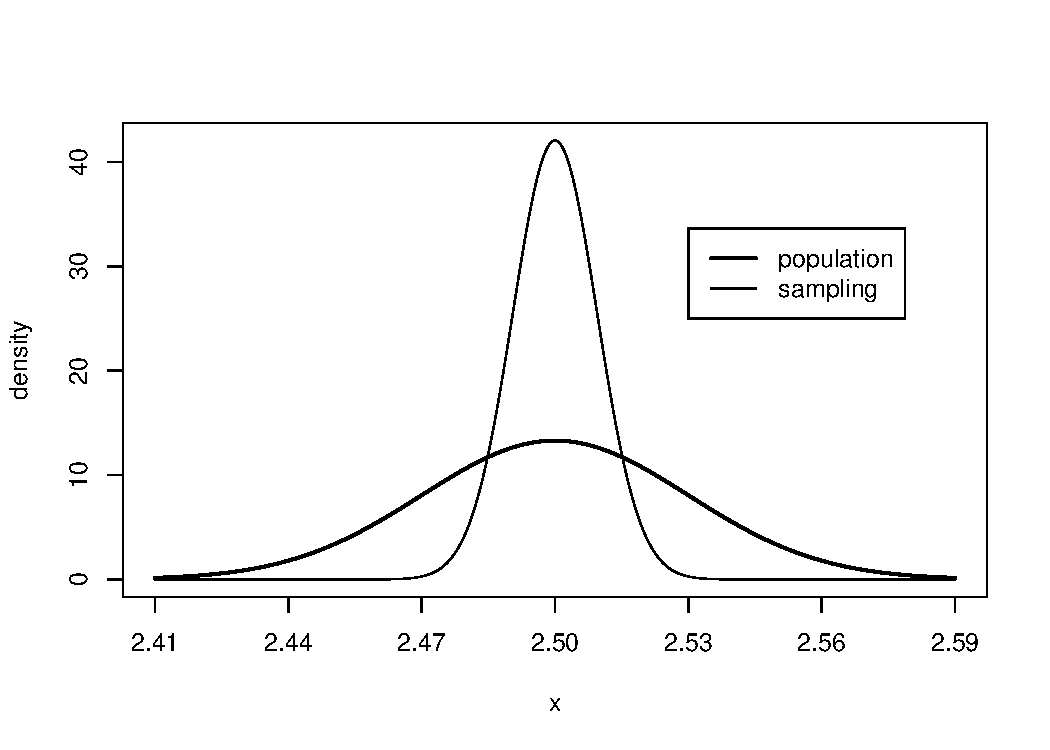
\includegraphics[scale=0.9]{code/Ex4p39_overlay.pdf}
\end{center}
\item We could not really estimate either. The population is not normal, and a sample size of 10 is not large enough to think the sampling distribution is normal.
\end{enumerate}


\newpage


\item \begin{enumerate}
\item We find a $z$ score.
$$z = \frac{10500-9000}{1000} = 1.5 $$
We find the probability.
$$P(X>10500) ~~=~~ P(Z>1.5) ~~=~~ 1-P(Z<1.5)~~=~~ 1-\Phi(1.5) ~~=~~ \fbox{0.067} $$
\item We need the standard error.
$$SE ~~=~~ \frac{1000}{\sqrt{15}} ~~=~~ 258.2 $$
A sampling distribution of a normal population is exactly normal with any sample size.
$$\bar{X} \sim \N{9000}{258} $$
\item We find the $z$-score.
$$z ~~=~~ \frac{10500-9000}{258} ~~=~~ 5.81 $$
This is a very large $z$-score... (Anything over 3.5 is very large.) 
$$P(\bar{X} > 10500) ~~=~~ P(Z>581) ~~\approx~~ 0  $$
\item {~}\\\vspace{-100pt}
\begin{center}
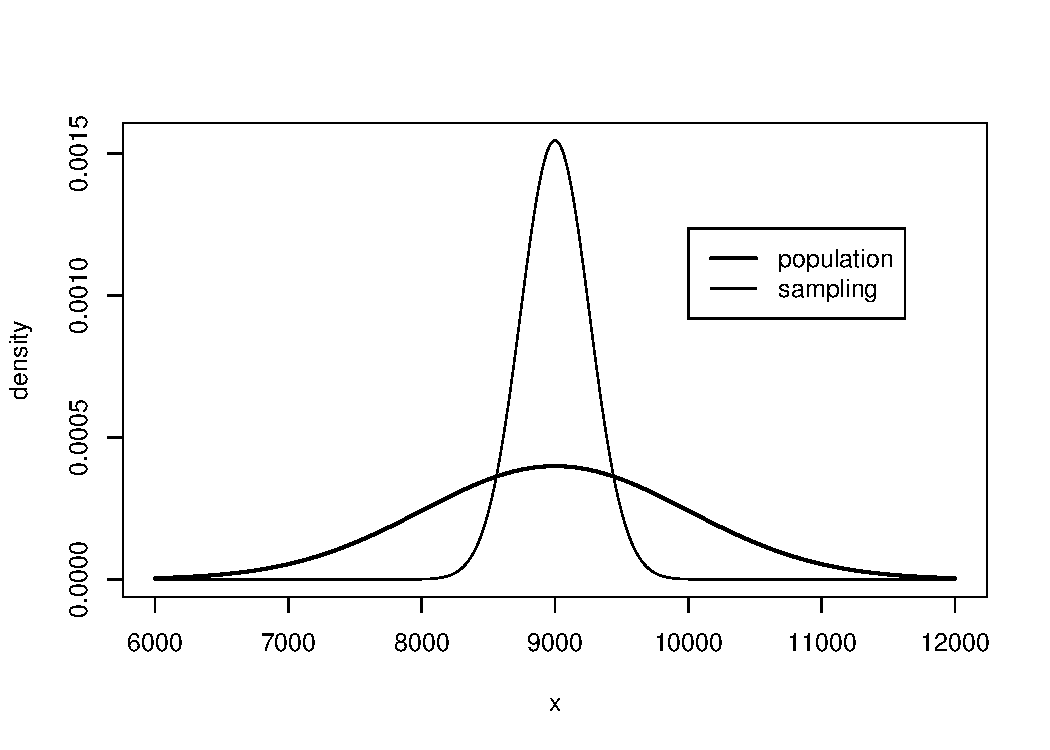
\includegraphics[scale=0.9]{code/Ex4p40_overlay.pdf}
\end{center}
\item Not unless we knew the population distribution. But we wouldn't be able to use normal approximations. Maybe the sampling distribution would still be almost normal is the skew was not strong.
\end{enumerate}


\newpage

\item \begin{enumerate}
\item We need to use the histogram. I'll estimate the heights of the bars corresponding to lengths over 5 minutes: 350, 100, 30, 30, 10. Thus, I estimate about 520 songs are over 5 minutes.
$$P(\text{song is over 5 minutes}) \approx \frac{520}{3000} = 0.173 $$
\item We find the minimum average length.
$$\frac{60}{15} = 4 $$
The population is not strongly skewed, so I bet the sampling distribution is almost normal. We let $\bar{X}\sim \N{3.45}{\frac{1.63}{\sqrt{15}}}$. Let's evaluate the standard error.
$$SE ~~=~~ \frac{1.63}{\sqrt{15}} ~~=~~ 0.42 $$
We calculate a $z$-score.
$$z ~~=~~ \frac{4-3.45}{0.42} ~~=~~ 1.31 $$
We find the appropriate probability.
$$P(\bar{X} > 4) ~~=~~ P(Z > 1.31) ~~=~~ 1-\Phi(0.62) ~~=~~0.095 $$
We think there is a 9.5\% chance of having enough music.

\item We determine the minimum average song length.
$$\frac{6 \times 60}{100} = 3.6 $$
We find the standard error.
$$SE = \frac{1.63}{\sqrt{100}} = 0.163 $$
We find the $z$-score.
$$z = \frac{3.6-3.45}{0.163} = 0.92$$
We find the probability.
$$P(\bar{X}>3.6) ~~=~~ P(Z>0.92) ~~=~~ 1-\Phi(0.92) ~~=~~ 0.179 $$
We think there is a 17.9\% chance the playlist will last the entire trip.
\end{enumerate}

\newpage

\item \begin{enumerate}
\item $z=\frac{27-25}{3}=0.67$
$$P(X>27) ~~=~~ P(Z>0.67) ~~=~~ 1-\Phi(0.67) ~~=~~ 0.25 $$
We think there is about a 25\% chance the can sprays more than 27 square feet.
\item 540/20=27.
\item We find the standard error.
$$SE = \frac{3}{\sqrt{20}} = 0.67 $$
We find the $z$ score.
$$\frac{27-25}{0.67} = 2.99$$
We find the probability.
$$P(\bar{X}>27) ~~=~~ P(Z>2.99) ~~=~~ 1-\Phi(2.99) ~~=~~ \fbox{0.0014} $$
\item We could not do (a) the same way. We might be able to get away with (c) since there is a slight skew.
\end{enumerate}

\end{enumerate}
\end{document}
